\documentclass[12pt]{article}
\usepackage[utf8]{vietnam}
\usepackage{amsmath}
\usepackage{amsfonts}
\usepackage{float}
\usepackage{fancyhdr}
\usepackage{graphicx}
\usepackage{svg}
\usepackage[colorlinks=true,linkcolor=blue, citecolor=red]{hyperref}
\usepackage{url}
\usepackage[top=.75in, left=.75in, right=.75in, bottom=1in]{geometry}
\usepackage{multirow}
\usepackage{enumitem}
\usepackage{setspace}
\usepackage{parskip}
\usepackage{tikz}
\usetikzlibrary{calc, fit, positioning, arrows.meta, shapes.geometric}
\usepackage{forest}
\usepackage{makecell}
% For algorithm
\usepackage{algorithm}
\usepackage{algpseudocode}

% For table
\usepackage{array}
\usepackage{diagbox}

% For references
\usepackage[backend=biber]{biblatex}
\addbibresource{ref/ref.bib}
\defbibheading{bibliography}[\refname]{}
\nocite{*}

% ============ CODE ============
\usepackage{listings}
\usepackage{xcolor}
\definecolor{codegreen}{rgb}{0,0.6,0}
\definecolor{codegray}{rgb}{0.5,0.5,0.5}
\definecolor{codepurple}{rgb}{0.58,0,0.82}
\definecolor{backcolour}{rgb}{0.95,0.95,0.92}

\lstdefinestyle{mystyle}{
    backgroundcolor=\color{backcolour},
    commentstyle=\color{codegreen},
    keywordstyle=\color{magenta},
    numberstyle=\tiny\color{codegray},
    stringstyle=\color{codepurple},
    basicstyle=\ttfamily\footnotesize,
    breakatwhitespace=false,
    breaklines=true,
    captionpos=b,
    keepspaces=true,
    numbers=left,
    numbersep=5pt,
    showspaces=false,
    showstringspaces=false,
    showtabs=false,
    tabsize=2
}
\lstset{style=mystyle}
\lstset{literate=%
% Vowel a
	{á}{{\'a}}1
	{à}{{\`a}}1
	{ạ}{{\d a}}1
	{ả}{{\h a}}1
	{ã}{{\~ a}}1
	{Á}{{\'A}}1
	{À}{{\`A}}1
	{Ạ}{{\d A}}1
	{Ả}{{\h A}}1
	{Ã}{{\~ A}}1
% Vowel breve-a
	{ă}{{\u a}}1
	{ắ}{{\'\abreve }}1
	{ằ}{{\`\abreve }}1
	{ặ}{{\d \abreve }}1
	{ẳ}{{\h \abreve }}1
	{ẵ}{{\~\abreve }}1
	{Ă}{{\u A}}1
	{Ắ}{{\'\ABREVE }}1
	{Ằ}{{\`\ABREVE }}1
	{Ặ}{{\d \ABREVE }}1
	{Ẳ}{{\h \ABREVE }}1
	{Ẵ}{{\~\ABREVE }}1
% Vowel circumflex-a
	{â}{{\^ a}}1
	{ấ}{{\'\acircumflex }}1
	{ầ}{{\`\acircumflex }}1
	{ậ}{{\d \acircumflex }}1
	{ẩ}{{\h \acircumflex }}1
	{ẫ}{{\~\acircumflex }}1
	{Â}{{\^ A}}1
	{Ấ}{{\'\ACIRCUMFLEX }}1
	{Ầ}{{\`\ACIRCUMFLEX }}1
	{Ậ}{{\d \ACIRCUMFLEX }}1
	{Ẩ}{{\h \ACIRCUMFLEX }}1
	{Ẫ}{{\~\ACIRCUMFLEX }}1
% Letter d-stroke
	{đ}{{\dj }}1
	{Đ}{{\DJ }}1
% Vowel e
	{é}{{\'e}}1
	{è}{{\`e}}1
	{ẹ}{{\d e}}1
	{ẻ}{{\h e}}1
	{ẽ}{{\~ e}}1
	{É}{{\'E}}1
	{È}{{\`E}}1
	{Ẹ}{{\d E}}1
	{Ẻ}{{\h E}}1
	{Ẽ}{{\~ E}}1
% Vowel circumflex-e
	{ê}{{\^e}}1
	{ế}{{\'\ecircumflex }}1
	{ề}{{\`\ecircumflex }}1
	{ệ}{{\d \ecircumflex }}1
	{ể}{{\h \ecircumflex }}1
	{ễ}{{\~\ecircumflex }}1
	{Ê}{{\^E}}1
	{Ế}{{\'\ECIRCUMFLEX }}1
	{Ề}{{\`\ECIRCUMFLEX }}1
	{Ệ}{{\d \ECIRCUMFLEX }}1
	{Ể}{{\h \ECIRCUMFLEX }}1
	{Ễ}{{\~\ECIRCUMFLEX }}1
% Vowel i
	{í}{{\'i}}1
	{ì}{{\`\i }}1
	{ị}{{\d i}}1
	{ỉ}{{\h i}}1
	{ĩ}{{\~\i }}1
	{Í}{{\'I}}1
	{Ì}{{\`I}}1
	{Ị}{{\d I}}1
	{Ỉ}{{\h I}}1
	{Ĩ}{{\~I}}1
% Vowel o
	{ó}{{\'o}}1
	{ò}{{\`o}}1
	{ọ}{{\d o}}1
	{ỏ}{{\h o}}1
	{õ}{{\~o}}1
	{Ó}{{\'O}}1
	{Ò}{{\`O}}1
	{Ọ}{{\d O}}1
	{Ỏ}{{\h O}}1
	{Õ}{{\~O}}1
% Vowel circumflex-o
	{ô}{{\^o}}1
	{ố}{{\'\ocircumflex }}1
	{ồ}{{\`\ocircumflex }}1
	{ộ}{{\d \ocircumflex }}1
	{ổ}{{\h \ocircumflex }}1
	{ỗ}{{\~\ocircumflex }}1
	{Ô}{{\^O}}1
	{Ố}{{\'\OCIRCUMFLEX }}1
	{Ồ}{{\`\OCIRCUMFLEX }}1
	{Ộ}{{\d \OCIRCUMFLEX }}1
	{Ổ}{{\h \OCIRCUMFLEX }}1
	{Ỗ}{{\~\OCIRCUMFLEX }}1
% Vowel horn-o
	{ơ}{{\ohorn }}1
	{ớ}{{\'\ohorn }}1
	{ờ}{{\`\ohorn }}1
	{ợ}{{\d \ohorn }}1
	{ở}{{\h \ohorn }}1
	{ỡ}{{\~\ohorn }}1
	{Ơ}{{\OHORN }}1
	{Ớ}{{\'\OHORN }}1
	{Ờ}{{\`\OHORN }}1
	{Ợ}{{\d \OHORN }}1
	{Ở}{{\h \OHORN }}1
	{Ỡ}{{\~\OHORN }}1
% Vowel u
	{ú}{{\'u}}1
	{ù}{{\`u}}1
	{ụ}{{\d u}}1
	{ủ}{{\h u}}1
	{ũ}{{\~u}}1
	{Ú}{{\'U}}1
	{Ù}{{\`U}}1
	{Ụ}{{\d U}}1
	{Ủ}{{\h U}}1
	{Ũ}{{\~U}}1
% Vowel horn-u
	{ư}{{\uhorn }}1
	{ứ}{{\'\uhorn }}1
	{ừ}{{\`\uhorn }}1
	{ự}{{\d \uhorn }}1
	{ử}{{\h \uhorn }}1
	{ữ}{{\~\uhorn }}1
	{Ư}{{\UHORN }}1
	{Ứ}{{\'\UHORN }}1
	{Ừ}{{\`\UHORN }}1
	{Ự}{{\d \UHORN }}1
	{Ử}{{\h \UHORN }}1
	{Ữ}{{\~\UHORN }}1
% Vowel y
	{ý}{{\'y}}1
	{ỳ}{{\`y}}1
	{ỵ}{{\d y}}1
	{ỷ}{{\h y}}1
	{ỹ}{{\~y}}1
	{Ý}{{\'Y}}1
	{Ỳ}{{\`Y}}1
	{Ỵ}{{\d Y}}1
	{Ỷ}{{\h Y}}1
	{Ỹ}{{\~Y}}1
}

% ============ DOCUMENT INFO ============
\newcommand{\reportname}{Seminar}
\newcommand{\coursetitle}{Phân Tích Dữ Liệu Thông Minh}
\newcommand{\coursename}{Phân Tích Dữ Liệu Thông Minh}
\newcommand{\teachername}{TS. Bùi Tiến Lên}
\newcommand{\studentname}{%
    Lê Duy Anh (22127012)\\
    Huỳnh Cao Tuấn Kiệt (22127219)\\
    Võ Thành Nghĩa (22127295)%
}

% ============ HEADER / FOOTER ============
\setlength{\headheight}{14.5pt}
\pagestyle{fancy}
\fancyhf{}
\fancyfoot[R]{\thepage}
\lhead{\reportname}
\rhead{\coursename}

% Set line and paragraph spacing
\renewcommand{\baselinestretch}{1.05}
\setlength{\parskip}{2pt}

% ============ DOCUMENT ============
\begin{document}
\begin{titlepage}
\newcommand{\HRule}{\rule{\linewidth}{0.5mm}}
\centering

\textsc{\LARGE đại học quốc gia thành phố hồ chí minh}\\[0.2cm]
\textsc{\LARGE trường đại học khoa học tự nhiên}\\[0.3cm]
\textsc{\Large khoa công nghệ thông tin}\\[0.5cm]


\includegraphics[scale=.35]{image/hcmus-logo.png}\\[0.5cm]

\huge{\bfseries{SEMINAR}}\\[0.3cm]
\Large{\bfseries{Double Machine Learning for Causal Inference}}\\
\Large{\bfseries{under Shared-State Interference}}\\[0.3cm]
\textbf{\large MÔN HỌC: \coursetitle}\\[0.5cm]

\begin{minipage}[t]{0.5\textwidth}
\begin{flushleft} \large
\emph{Sinh viên thực hiện:}\\
\studentname
\end{flushleft}
\end{minipage}
~
\begin{minipage}[t]{0.4\textwidth}
\begin{flushright} \large
\emph{Giảng viên:} \\
\teachername
\end{flushright}
\end{minipage}\\[4cm]

{\large \today}\\[2cm]


\vfill
\end{titlepage}
	

\tableofcontents
\pagebreak
\section{Thông tin chung}

\subsection{Thông tin bài báo}

\begin{itemize}
    \item Tên bài báo: Double Machine Learning for Causal Inference under Shared-State Interference
    \item Tác giả: Chris Hays \& Manish Raghavan
    \item Đơn vị: Massachusetts Institute of Technology (MIT)
    \item Hội nghị: International Conference on Machine Learning (ICML 2025)
    \item Mã arXiv: \href{https://arxiv.org/abs/2504.08836}{arXiv:2504.08836v1}
\end{itemize}

\subsection{Tóm tắt nội dung}

Bài báo giải quyết bài toán suy luận nhân quả (causal inference) trong các hệ thống mà giả định không nhiễu loạn (SUTVA) bị vi phạm. Cụ thể, nhiều nền tảng thực tế như hệ thống gợi ý, sàn thương mại điện tử, ứng dụng gọi xe có đặc điểm: hành động của một người dùng tác động lên một trạng thái chung (shared state) và từ đó ảnh hưởng đến kết quả của những người dùng khác. Dạng nhiễu loạn có cấu trúc này được tác giả đặt tên là Shared-State Interference (SSI).

Thách thức nằm ở chỗ trạng thái chung $H_t$ vừa phụ thuộc vào lịch sử đối xử, vừa trực tiếp chi phối kết quả, tạo ra mối quan hệ phụ thuộc phức tạp theo chuỗi thời gian mà các phương pháp DML truyền thống (vốn giả định dữ liệu i.i.d.) không thể xử lý đúng đắn.

Đóng góp cốt lõi của bài báo bao gồm:

\begin{enumerate}
    \item Khung lý thuyết tổng quát cho SSI: Hình thức hóa mô hình SSI với chuỗi quan sát $\{(X_t, D_t, H_t, Y_t)\}_{t=1}^{T}$, trong đó $H_t$ đóng vai trò trung gian (mediator) cho mọi tác động lan tỏa.

    \item Mở rộng DML sang dữ liệu phụ thuộc: Đề xuất bộ ước lượng semiparametric, kết hợp học máy linh hoạt (nuisance estimation) với phép chiếu Frisch-Waugh-Lovell, đồng thời chứng minh tính chuẩn tiệm cận (asymptotic normality) ngay cả khi các quan sát tương quan theo thời gian.

    \item Bộ ước lượng phương sai nhất quán: Xây dựng ước lượng phương sai (HAC-style) từ mixing conditions phù hợp với chuỗi SSI, cho phép tạo khoảng tin cậy có độ phủ đúng trong thực tế.
\end{enumerate}

Kết quả mô phỏng cho thấy phương pháp DML4SSI đạt độ phủ khoảng tin cậy xấp xỉ 95\% và độ lệch gần bằng 0, trong khi các baseline ngây thơ (plug-in, HT, DML i.i.d.) đều bị chệch đáng kể.

\section{Đặt vấn đề và Động lực}

\subsection{Hiện tượng Nhiễu loạn (Interference) và SUTVA}

Suy luận nhân quả truyền thống dựa trên giả định \textbf{không có nhiễu loạn giữa các đơn vị (Stable Unit Treatment Value Assumption --- SUTVA)}: kết quả của một đơn vị không bị ảnh hưởng bởi đối xử của đơn vị khác. Tuy nhiên, giả định này sụp đổ trong nhiều hệ thống thực tế:

\begin{itemize}
    \item \textbf{Hệ thống gợi ý:} Tương tác của một người dùng làm thay đổi nội dung gợi ý cho những người dùng sau (trạng thái chung: điểm phổ biến, embedding, lịch sử xem).
    \item \textbf{Thị trường / Sàn thương mại điện tử:} Khuyến mãi cho một nhóm người dùng làm thay đổi nhu cầu, giá cả, thời gian chờ và hàng tồn kho (trạng thái chung: lượng tồn kho, giá hiện tại, tín hiệu cầu).
    \item \textbf{Gọi xe công nghệ:} Đối xử với một số hành khách làm thay đổi lượng tài xế trống cho những người khác (trạng thái chung: số tài xế trống, giá linh động, thời gian chờ).
\end{itemize}

Ngay cả \textit{thí nghiệm ngẫu nhiên (randomized experiments)} cũng có thể bị chệch khi một đơn vị được đối xử làm thay đổi điều kiện thị trường chung, ảnh hưởng đến các đơn vị sau.

\subsection{Khái niệm Nhiễu loạn Trạng thái chung (Shared-State Interference)}

Bài báo đề xuất một dạng nhiễu loạn có cấu trúc, được gọi là \textbf{Shared-State Interference (SSI)}: nhiễu loạn không tùy tiện mà chảy qua một trạng thái chung quan sát được \(H_t\), thứ tóm gọn toàn bộ tác động lan tỏa (spillover) trong quá khứ.

\(H_t\) có thể là lượng hàng tồn kho, giá cả, thời gian chờ, điểm phổ biến, hay đầu ra của thuật toán gợi ý --- bất kỳ cơ chế nào trung chuyển tác động lan tỏa giữa các đơn vị theo thời gian. Các đơn vị vừa \textit{bị ảnh hưởng} bởi trạng thái chung, vừa \textit{góp phần làm thay đổi} nó.

Cấu trúc phụ thuộc của SSI được tóm tắt như sau:
\[
    W_{t-1} \;\longrightarrow\; H_t \;\longrightarrow\; Y_t
\]
Quá khứ chỉ ảnh hưởng tương lai thông qua trạng thái chung \(H_t\), không có mũi tên ngang nối trực tiếp giữa các đơn vị.

\subsection{Hạn chế của nghiên cứu trước và Đóng góp của bài báo}

Các nghiên cứu trước đây về nhiễu loạn thường dựa vào mô hình \textbf{tham số cố định (parametric)}, hoặc giả định đặc thù cho từng bài toán cụ thể, dẫn đến dễ bị chệch khi mô hình hóa sai và khó mở rộng sang bối cảnh khác.

Bài báo của Hays và Raghavan (2025) đóng góp ba điểm chính:

\begin{enumerate}
    \item Đưa ra \textbf{khung lý thuyết tổng quát (General Framework)} cho SSI, không phụ thuộc vào giả định tham số cụ thể.
    \item Mở rộng định lý \textbf{Double Machine Learning (DML) cho SSI} --- sử dụng các mô hình học máy linh hoạt, semiparametric, vẫn đảm bảo suy luận thống kê hợp lệ trên dữ liệu phụ thuộc.
    \item Cung cấp \textbf{bộ ước lượng phương sai nhất quán (Consistent Variance Estimator)} để xây dựng khoảng tin cậy chính xác ngay cả khi các quan sát có tương quan theo thời gian.
\end{enumerate}

Điểm mấu chốt: kết hợp được tính linh hoạt của học máy với suy luận thống kê hợp lệ, ngay cả khi dữ liệu phụ thuộc theo chuỗi thời gian.

\section{Mô hình hóa Shared-State Interference}

\subsection{Thiết lập mô hình toán học (Setting \& Notation)}

Xét một chuỗi các đơn vị được lập chỉ số \(t = 1, 2, \dots, T\). Tại mỗi bước thời gian \(t\), ta quan sát bộ dữ liệu:
\[
    W_t = \{X_t,\, D_t,\, H_t,\, Y_t\}
\]

Trong đó:
\begin{itemize}
    \item \(X_t\): \textbf{biến nền cảnh (covariates)} độc lập đồng phân phối (i.i.d.) từ không gian mẫu \(\mathbb{R}^{p_X}\) --- ví dụ vị trí, lịch sử xem, thiết bị.
    \item \(D_t \in \{0, 1\}\): \textbf{biến đối xử nhị phân (binary treatment)}, độc lập với dữ liệu quá khứ nhưng có thể phụ thuộc vào \(X_t\).
    \item \(H_t \in \mathbb{R}^{p_H}\): \textbf{trạng thái chung (shared state)} quan sát được --- biến cốt lõi của bài báo, tiến hóa theo thời gian theo dạng chuỗi Markov.
    \item \(Y_t(D_t, H_t)\): \textbf{kết quả tiềm năng (potential outcome)}, phụ thuộc vào \textit{hai} đối số: đối xử của chính đơn vị và trạng thái chung.
\end{itemize}

Khác với SUTVA (kết quả chỉ phụ thuộc \(D_t\)), ở đây \(Y_t\) bị đồng quyết định bởi cả \(D_t\) lẫn trạng thái chung \(H_t\). Tồn tại vòng lặp phản hồi hai chiều: \(H_t \to Y_t\), và ngược lại \((D_t, X_t) \to H_{t+1}\). Cấu trúc phụ thuộc này được minh họa trong Hình~\ref{fig:dag-ssi}.

\begin{figure}[H]
\centering
\begin{tikzpicture}[
    node distance = 1.4cm and 1.8cm,
    every node/.style = {font=\small},
    var/.style = {draw, rectangle, rounded corners=4pt, minimum width=1.1cm,
                  minimum height=0.75cm, fill=gray!10, thick},
    shared/.style = {draw, ellipse, minimum width=2.2cm, minimum height=1.2cm,
                     fill=blue!15, draw=blue!70, thick},
    outcome/.style = {draw, circle, minimum size=1.1cm,
                      fill=green!20, draw=green!60!black, thick},
    groupbox/.style = {draw, dashed, rounded corners=6pt, gray, thick, inner sep=8pt},
    arr/.style  = {->, >=stealth, thick, blue!70},
    garr/.style = {->, >=stealth, thick, gray!60},
]
% W_{t-1} group
\node[var] (Xt1) {$X_{t-1}$};
\node[var, below=0.35cm of Xt1] (Dt1) {$D_{t-1}$};
\node[var, below=0.35cm of Dt1] (Yt1) {$Y_{t-1}$};
\node[var, below=0.35cm of Yt1, fill=blue!10, draw=blue!50] (Ht1) {$H_{t-1}$};
\node[groupbox, fit=(Xt1)(Ht1),
      label={[gray,font=\scriptsize]above:$W_{t-1}$}] (Wt1) {};

% H_t shared state
\node[shared, right=2.6cm of Dt1] (Ht) {};
\node[font=\footnotesize\itshape, blue!80, above] at (Ht.center) {trạng thái chung};
\node[font=\bfseries, blue!90!black, below] at (Ht.center) {$H_t$};

% X_t, D_t
\node[var, above right=0.5cm and 2.0cm of Ht] (Xt) {$X_t$};
\node[var, below right=0.5cm and 2.0cm of Ht] (Dt) {$D_t$};

% Y_t
\node[outcome] at ($(Xt)!0.5!(Dt) + (1.8cm,0)$) (Yt) {$Y_t$};

% Arrows
\draw[arr]  (Wt1.east) -- (Ht);
\draw[arr]  (Ht) -- (Yt);
\draw[garr] (Xt)  -- (Yt);
\draw[garr] (Dt)  -- (Yt);
\end{tikzpicture}
\caption{Cấu trúc phụ thuộc của Shared-State Interference. Quá khứ \(W_{t-1}\) ảnh hưởng tương lai chỉ thông qua trạng thái chung \(H_t\). Các đơn vị không tương tác trực tiếp mà gián tiếp qua \(H_t\).}
\label{fig:dag-ssi}
\end{figure}

\subsection{Tính chất Markov của Trạng thái chung}

Giả định cốt lõi của bài báo là trạng thái chung \(H_t\) thỏa mãn tính chất Markov:

\begin{equation}
    P(H_t \in A \mid W_{1:t-1}) = P(H_t \in A \mid W_{t-1}) \tag{2.1}
\end{equation}

Khi đã biết quan sát ngay trước đó \(W_{t-1}\), trạng thái chung kế tiếp \(H_t\) độc lập điều kiện với toàn bộ lịch sử xa hơn --- ``quá khứ xa đã được gói gọn trong hiện tại''.

Do \(X_t\) i.i.d. và \(D_t\) không phụ thuộc quá khứ, toàn chuỗi \(\{W_t\}\) tạo thành một \textbf{chuỗi Markov thuần nhất (homogeneous Markov chain)} với kernel chuyển trạng thái \(K_H\) cố định --- nền móng để áp dụng các định lý giới hạn trong phần sau.

\subsection{Các điều kiện của Chuỗi Markov (Assumption 2.1)}

Hệ thống SSI phải thỏa mãn \textbf{một trong hai} cấu trúc phụ thuộc sau:

\paragraph{Điều kiện (a) --- Hội tụ hình học (Geometric Ergodicity):}
Chuỗi Markov hội tụ về một phân phối dừng duy nhất với tốc độ hàm mũ. Nói nôm na: ``nhiễu phai nhạt nhanh theo hàm mũ'' --- tương quan giữa các quan sát cách xa nhau giảm về 0 đủ nhanh để suy luận tiệm cận có hiệu lực. Điều kiện này phù hợp với bài toán dữ liệu quan sát (observational data).

\paragraph{Điều kiện (b) --- Phụ thuộc hữu hạn (\(m\)-Dependence):}
Các quan sát cách nhau xa hơn \(m\) bước thì hoàn toàn độc lập:
\[
    W_{1:t} \perp W_{t+m+1:T}
\]
Nói nôm na: ``nhiễu chỉ kéo dài tối đa \(m\) bước rồi biến mất''. Điều kiện này tự nhiên xuất hiện trong các thử nghiệm Switchback.

Hai điều kiện này \textit{thay thế} giả định i.i.d.\ trong DML thông thường, cho phép một Định lý Giới hạn Trung tâm (CLT) vẫn đúng trên dữ liệu phụ thuộc. Tương ứng với hai điều kiện này, bài báo cũng đề xuất hai công thức ước lượng phương sai khác nhau.

\section{Lý thuyết Double Machine Learning cho SSI}

\subsection{Mô hình bài toán}

Mô hình cơ bản của bài báo là:
\[
    Y_t = \theta_0\, D_t + g_0(X_t) + \varepsilon_t
\]

Trong đó:
\begin{itemize}
    \item \(\theta_0\): \textbf{tác động điều trị (treatment effect)} cần ước lượng. Ký hiệu \(_0\) chỉ \textit{giá trị thực ở tổng thể (true value)}.
    \item \(g_0(X_t)\): \textbf{hàm nhiễu (nuisance function)} --- kỳ vọng điều kiện của các yếu tố gây nhiễu lên kết quả; phi tuyến và không biết trước.
    \item \(\varepsilon_t\): nhiễu ngẫu nhiên.
\end{itemize}

Mục tiêu duy nhất là ước lượng \(\theta_0\) một cách \textbf{không chệch}, dù \(g_0\) phức tạp và phải học bằng máy. Khi có trạng thái chung \(H_t\), mô hình mở rộng thành:
\[
    Y_t = \theta_0\, D_t + g_0(X_t, H_t) + \varepsilon_t
\]

\subsection{Ý tưởng cốt lõi: Định lý Frisch-Waugh-Lovell (FWL)}

DML tìm tác động điều trị dựa trên ý tưởng từ \textbf{Định lý Frisch-Waugh-Lovell}: trong hồi quy tuyến tính, \(\theta_0\) có thể được cô lập bằng cách làm sạch ảnh hưởng của \(X\) khỏi cả \(Y\) lẫn \(D\).

\textbf{Bước 1 --- Làm sạch \(Y\):}
\begin{enumerate}
    \item Hồi quy \(Y\) theo \(X\) để thu được dự đoán \(\hat{l}(X_t, H_t) \approx \mathbb{E}[Y \mid X, H]\)
    \item Tính phần dư: \(\tilde{Y}_t = Y_t - \hat{l}(X_t, H_t)\)
\end{enumerate}

\textbf{Bước 2 --- Làm sạch \(D\):}
\begin{enumerate}
    \item Hồi quy \(D\) theo \(X\) để thu được propensity score \(\hat{m}(X_t) \approx \mathbb{E}[D \mid X]\)
    \item Tính phần dư: \(\tilde{D}_t = D_t - \hat{m}(X_t)\)
\end{enumerate}

\textbf{Bước 3 --- Hồi quy phần dư:} Hồi quy \(\tilde{Y}\) theo \(\tilde{D}\):
\[
    \tilde{Y}_t = \theta_0\, \tilde{D}_t + u_t \implies \hat{\theta} \xrightarrow{p} \theta_0
\]

DML (Chernozhukov et al., 2018) tổng quát hóa ý tưởng này: thay vì dùng hồi quy tuyến tính để làm sạch, sử dụng các mô hình học máy linh hoạt.

\subsection{Vấn đề khi Cross-Fitting gặp SSI}

Trong DML thông thường, \textbf{cross-fitting (K-fold)} được dùng để tránh overfitting: học mô hình trên các fold train, tính phần dư trên fold test còn lại. Tuy nhiên, khi có trạng thái chung \(H_t\), cross-fitting không còn hợp lệ vì hai lý do:

\paragraph{Vấn đề 1 --- Data Leakage qua \(H_t\):}
\(H_t\) được tính từ \(W_{t-1} = (D_{t-1}, Y_{t-1}, H_{t-1})\) --- toàn bộ thông tin của bước liền trước. Khi bước \(t\) thuộc fold test nhưng bước \(t-1\) thuộc fold train, bộ ước lượng \(\hat{l}, \hat{m}\) đã gián tiếp ``thấy'' quan sát test thông qua \(H_t\). Phần dư \(\tilde{Y}_t\) bị thu hẹp giả tạo (overfit), kéo \(\hat{\theta}\) về phía 0 --- \textbf{ước lượng bị chệch}.

\paragraph{Vấn đề 2 --- Lệch phương sai ước lượng:}
\(H_t\) tạo \textbf{tương quan chuỗi} giữa các hàm score \(\phi_t\), khiến công thức phương sai DML thông thường (chỉ tính phần tổng phương sai, bỏ qua hiệp phương sai) trở nên sai lệch:
\[
    \operatorname{Var}(\hat{\theta}) = \frac{1}{T}\sum_t \operatorname{Var}(\phi_t) + \frac{2}{T}\sum_{t < s} \operatorname{Cov}(\phi_t, \phi_s)
\]
Bỏ qua phần \(\operatorname{Cov}\) làm khoảng tin cậy và \(p\)-value \textbf{không còn hiệu lực}.

\begin{figure}[H]
    \centering
    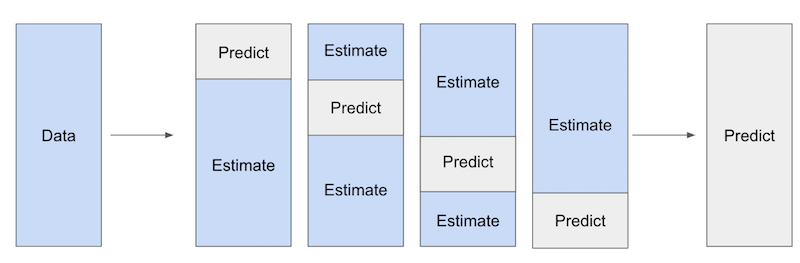
\includegraphics[width=0.78\textwidth]{image/cross-prediction.png}
    \caption{Minh họa cross-fitting K-fold: mỗi fold lần lượt được giữ lại để \textbf{Predict} (test); các fold còn lại dùng để \textbf{Estimate} (học \(\hat{l}, \hat{m}\)). Phần dư out-of-fold không bị overfit vì mô hình chưa từng thấy quan sát đó.}
    \label{fig:cross-fitting}
\end{figure}

\subsection{Giải pháp 1: Auxiliary Data (Dữ liệu phụ trợ độc lập)}

Thay vì cross-fitting, bài báo đề xuất dùng một tập dữ liệu phụ trợ \(W_{\text{aux}}\) \textbf{độc lập} với tập suy luận \(W_{1:T}\):

\begin{algorithm}[H]
\caption{Double Machine Learning for Shared-State Interference (DML4SSI)}
\begin{algorithmic}[1]
    \State \textbf{Bước 1:} Học nuisance functions \(\hat{\eta} = (\hat{l}, \hat{m})\) từ \(W_{\text{aux}}\)
    \State \textbf{Bước 2:} Áp \(\hat{l}, \hat{m}\) lên \(W_{1:T}\) để tính phần dư \(\tilde{Y}_t, \tilde{D}_t\)
    \State \textbf{Bước 3:} Tính \(\hat{\psi} \stackrel{\text{def}}{=} \psi(W_{1:T}, \hat{\eta})\) --- hồi quy phần dư
    \State \Return \(\hat{\psi}\)
\end{algorithmic}
\end{algorithm}

Vì \(W_{\text{aux}} \perp W_{1:T}\), phần dư \(\tilde{Y}, \tilde{D}\) không bị overfit, đảm bảo \(\hat{\theta}\) tiệm cận không lệch dù \(H_t\) phụ thuộc theo thời gian.

\begin{figure}[H]
\centering
\begin{tikzpicture}[
    font=\small,
    box/.style={draw, rounded corners=5pt, thick, minimum height=1.6cm,
                text width=#1, align=center, inner sep=6pt},
    arr/.style={->, >=stealth, thick},
    perp/.style={draw, dashed, green!60!black, rounded corners=5pt, thick,
                 inner sep=6pt, fill=green!6},
]

% ── Top row ──────────────────────────────────────────────────
\node[box=2.0cm, fill=blue!15, draw=blue!60] (Waux) at (0,0) {
    \textbf{Tập phụ trợ}\\[2pt]
    $W_{\text{aux}}$\\[2pt]
    {\footnotesize\itshape độc lập với $W_{1:T}$}
};

\node[box=4.2cm, fill=gray!15, draw=gray!50, right=1.0cm of Waux] (step1) {
    \textbf{Bước 1 · Train nuisance $\hat{\eta}$}\\[4pt]
    \begin{tabular}{cc}
        \colorbox{blue!25}{$\hat{l}(X_t,H_t)$} & \colorbox{violet!20}{$\hat{m}(X_t,H_t)$} \\[2pt]
        {\tiny outcome model} & {\tiny propensity model}
    \end{tabular}
};

\node[perp, right=0.8cm of step1, minimum height=1.6cm, text width=2.2cm, align=center] (badge) {
    {\small $W_{\text{aux}} \perp W_{1:T}$}\\[3pt]
    {\footnotesize $\hat{\eta}$ không thấy $W_{1:T}$}\\
    {\footnotesize $\Rightarrow$ phần dư không overfit}
};

\draw[arr, blue!60] (Waux) -- node[above,font=\scriptsize]{train} (step1);

% ── Down arrow ───────────────────────────────────────────────
\node[below=0.5cm of step1, font=\scriptsize, blue!70] (lbl) {apply $\hat{\eta}$ lên $W_{1:T}$};
\draw[arr, blue!70] (step1.south) -- (lbl.north);

% ── Bottom row ───────────────────────────────────────────────
\node[box=2.0cm, fill=orange!15, draw=orange!60, below=0.9cm of Waux] (W1T) {
    \textbf{Tập chính}\\[2pt]
    $W_{1:T}$\\[2pt]
    {\footnotesize\itshape chuỗi Markov}
};

\node[box=4.2cm, fill=yellow!20, draw=yellow!60!black, right=1.0cm of W1T] (step2) {
    \textbf{Bước 2 · Tính phần dư}\\[4pt]
    $\tilde{Y}_t = Y_t - \hat{l}(X_t,H_t)$\\[2pt]
    $\tilde{D}_t = D_t - \hat{m}(X_t,H_t)$
};

\node[box=2.2cm, fill=green!15, draw=green!60!black, right=1.0cm of step2] (step3) {
    \textbf{Bước 3}\\[2pt]
    $\tilde{Y}_t = \hat{\theta}\,\tilde{D}_t + u_t$\\[4pt]
    $\hat{\theta} \xrightarrow{p} \theta_0$
};

\draw[arr, orange!70] (W1T) -- (step2);
\draw[arr, yellow!60!black] (step2) -- (step3);
\draw[arr, blue!70] (lbl.south) -- (step2.north);

\end{tikzpicture}
\caption{Pipeline Auxiliary Data cho DML4SSI. Vì \(\hat{l}, \hat{m}\) được học từ \(W_{\text{aux}} \perp W_{1:T}\), phần dư \(\tilde{Y}, \tilde{D}\) không bị overfit và \(\hat{\theta}\) tiệm cận không lệch.}
\label{fig:aux-pipeline}
\end{figure}

\subsection{Giải pháp 2: Block Cross-Fitting với khoảng đệm (\textit{m}-Dependence)}

Nếu các quan sát cách nhau hơn \(m\) bước là độc lập hoàn toàn, ta có thể chia dữ liệu thành các khối liên tục và chèn \textbf{khoảng đệm \(m\)} giữa train và test để chặn rò rỉ qua \(H_t\):

\begin{itemize}
    \item Chia \(W_{1:T}\) thành \(K\) khối liên tục
    \item Mỗi lượt: một khối làm test, các khối còn lại làm train
    \item Bỏ qua \(m\) quan sát đầu tiên của khối liền sau test để đảm bảo \(H_t\) đã ``phai'' đủ
\end{itemize}

Điều kiện áp dụng: cần biết \(m\) --- khoảng thời gian để \(H_t\) phai nhạt hoàn toàn. Đây là phương pháp phổ biến với thử nghiệm switchback trong thực tế (Uber, Lyft, Netflix).

\begin{figure}[H]
\centering
% Grid layout (all measurements in cm):
%   Label area : x = 0..1.2  (anchor east at 1.2)
%   Col 1      : x = 1.3..4.3  (width 3.0, center 2.80)
%   Col 2      : x = 4.5..7.5  (width 3.0, center 6.00)
%   Col 3      : x = 7.7..10.7 (width 3.0, center 9.20)
%   Split dims : gap = 0.65 cm, train-portion = 2.35 cm
%   Split centers "gap|train" at col_left L:
%     gap   = L + 0.325,  train = L + 1.825
%   Split centers "train|gap" at col_left L:
%     train = L + 1.175,  gap   = L + 2.675
%   Rows       : y = 0.0, -1.0, -2.0  (spacing 1.0 cm)
\begin{tikzpicture}[font=\small]
\tikzset{
    TB/.style={draw=blue!70, fill=blue!25, thick, minimum height=0.70cm,
               rounded corners=3pt, align=center,
               font=\footnotesize\bfseries, text=blue!80!black},
    TS/.style={draw=green!60!black, fill=green!20, thick, minimum height=0.70cm,
               rounded corners=3pt, align=center,
               font=\footnotesize\bfseries, text=green!40!black},
    GB/.style={draw=gray!50, fill=gray!15, thick, minimum height=0.70cm,
               rounded corners=2pt, align=center,
               font=\scriptsize\bfseries, text=gray!60},
    LBL/.style={font=\footnotesize\bfseries, anchor=east},
    CLH/.style={font=\footnotesize\itshape, gray},
}

% Column headers
\node[CLH] at (2.80,  0.55) {Khối 1};
\node[CLH] at (6.00,  0.55) {Khối 2};
\node[CLH] at (9.20,  0.55) {Khối 3};

% Thin vertical dividers
\draw[gray!25, thin] (4.40,  0.45) -- (4.40, -2.40);
\draw[gray!25, thin] (7.60,  0.45) -- (7.60, -2.40);

%── Lượt 1: Test(full) | gap(0.65)+Train(2.35) | Train(full) ──
\node[LBL] at (1.20,  0.00) {Lượt 1};
\node[TS, minimum width=3.00cm] at (2.800,  0.00) {Test 1};   % Col1 full
\node[GB, minimum width=0.65cm] at (4.825,  0.00) {$m$};      % Col2 gap  L=4.5→4.5+0.325
\node[TB, minimum width=2.35cm] at (6.325,  0.00) {Train};    % Col2 train L=4.5→4.5+1.825
\node[TB, minimum width=3.00cm] at (9.200,  0.00) {Train};    % Col3 full

%── Lượt 2: Train(2.35)+gap(0.65) | Test(full) | gap(0.65)+Train(2.35) ──
\node[LBL] at (1.20, -1.00) {Lượt 2};
\node[TB, minimum width=2.35cm] at (2.475, -1.00) {Train};    % Col1 train L=1.3→1.3+1.175
\node[GB, minimum width=0.65cm] at (3.975, -1.00) {$m$};      % Col1 gap   L=1.3→1.3+2.675
\node[TS, minimum width=3.00cm] at (6.000, -1.00) {Test 2};   % Col2 full
\node[GB, minimum width=0.65cm] at (8.025, -1.00) {$m$};      % Col3 gap   L=7.7→7.7+0.325
\node[TB, minimum width=2.35cm] at (9.525, -1.00) {Train};    % Col3 train L=7.7→7.7+1.825

%── Lượt 3: Train(full) | Train(2.35)+gap(0.65) | Test(full) ──
\node[LBL] at (1.20, -2.00) {Lượt 3};
\node[TB, minimum width=3.00cm] at (2.800, -2.00) {Train};    % Col1 full
\node[TB, minimum width=2.35cm] at (5.675, -2.00) {Train};    % Col2 train L=4.5→4.5+1.175
\node[GB, minimum width=0.65cm] at (7.175, -2.00) {$m$};      % Col2 gap   L=4.5→4.5+2.675
\node[TS, minimum width=3.00cm] at (9.200, -2.00) {Test 3};   % Col3 full

%── Legend ─────────────────────────────────────────────────────
\node[TB, minimum width=1.0cm] at (2.50, -2.85) {};
\node[font=\footnotesize, anchor=west] at (3.05, -2.85) {Train};
\node[TS, minimum width=1.0cm] at (5.50, -2.85) {};
\node[font=\footnotesize, anchor=west] at (6.05, -2.85) {Test};
\node[GB, minimum width=1.0cm] at (8.20, -2.85) {$m$};
\node[font=\footnotesize, anchor=west] at (8.75, -2.85) {Khoảng đệm};

\end{tikzpicture}
\caption{Block Cross-Fitting với khoảng đệm \(m\). Mỗi lượt giữ một khối làm Test; khoảng đệm \(m\) bước (\textcolor{gray}{xám}) ngăn cách Test khỏi khối Train liền kề, đảm bảo \(H_t\) đã phai hoàn toàn.}
\label{fig:block-crossfit}
\end{figure}

\subsection{Định lý chính (Theorem 3.3)}

\subsubsection{Các giả định cần thiết}

Ngoài hai giả định về cấu trúc chuỗi Markov (Assumption 2.1a/b), định lý yêu cầu thêm hai điều kiện:

\paragraph{Assumption 3.1 --- Neyman Orthogonality (Trực giao Neyman):}
Đạo hàm Gateaux bậc nhất của \(\psi\) theo \(\eta\) tại giá trị thực \(\eta^*\), đánh giá theo mọi hướng \(\eta \in S_T\), bằng 0:
\[
    \partial_r \,\mathbb{E}_P\bigl[\psi(W_{1:T};\, \eta^* + r(\eta - \eta^*))\bigr]\big|_{r=0} = 0
\]
Điều kiện này đảm bảo rằng sai số ước lượng nuisance \(\hat{\eta} - \eta^*\) chỉ gây ra \textbf{sai lệch bậc hai} (second-order bias) lên \(\hat{\psi}\), chứ không phải bậc nhất. Nhờ đó, dù \(\hat{\eta}\) hội tụ chậm hơn tốc độ tham số, \(\hat{\psi}\) vẫn đạt tốc độ \(\sqrt{T}\).

\paragraph{Assumption 3.2 --- Điều kiện hội tụ (Convergence rate conditions):}
Tồn tại các hằng số \(\gamma, \delta, C > 0\) và \(T_0 \geq 1\) sao cho với mọi \(T > T_0\), bộ ước lượng nuisance \(\hat{\eta}(W_{\text{aux}})\) thuộc tập hiện thực hóa \(S_T\) (chứa \(\eta^*\)) với xác suất ít nhất \(1 - \gamma\), trong đó \(S_T\) phải thỏa mãn:
\begin{align}
    \sup_{\eta \in S_T} \|\phi(W_t;\, \eta)\|_{L^{4+\delta}(P)} &< C, \quad \forall t \in [T] \tag{3.1}\\
    \sup_{\eta \in S_T} T^{-1} \sum_{t=1}^T \|\phi(W_t;\, \eta) - \phi(W_t;\, \eta^*)\|_{L^2(P)} &= o(1) \tag{3.2}\\
    \sup_{r \in (0,1),\, \eta \in S_T} \left|\partial^{(2)}_r \,\mathbb{E}_P\bigl[\psi(W_{1:T};\, \eta^* + r(\eta - \eta^*))\bigr]\right| &= o(T^{-1/2}) \tag{3.3}
\end{align}

Điều kiện (3.1) yêu cầu hàm score bị chặn trong chuẩn \(L^{4+\delta}\). Điều kiện (3.2) yêu cầu \(\hat{\eta}\) xấp xỉ \(\eta^*\) đồng đều theo thời gian. Điều kiện (3.3) --- quan trọng nhất --- yêu cầu đạo hàm bậc hai của \(\psi\) phải có cỡ \(o(T^{-1/2})\), tức tích tốc độ hội tụ của hai nuisance functions phải thỏa:
\[
    \|\hat{l} - l^*\|_{L^2} \cdot \|\hat{m} - m^*\|_{L^2} = o_P(T^{-1/2})
\]
Điều này cho phép mỗi mô hình học máy hội tụ chậm hơn tốc độ \(T^{-1/4}\) riêng lẻ, miễn là \textit{tích} của hai tốc độ đủ nhanh.

\subsubsection{Phát biểu định lý và hội tụ}

\textbf{Theorem 3.3:} Dưới Assumptions 2.1, 3.1 và 3.2, với xác suất không nhỏ hơn \(1 - \gamma\):
\[
    \sqrt{T}\, \hat{\sigma}^{-1} \bigl(\psi(W_{1:T};\, \hat{\eta}) - \psi^*\bigr) \xrightarrow{d} \mathcal{N}(0,\, 1)
\]

Tức là \(\hat{\psi}\) hội tụ về \(\psi^*\) ở tốc độ tham số \(\sqrt{T}\) và phân phối sai số chuẩn hóa hội tụ về chuẩn tắc.

\subsubsection{Vai trò của hai giả định Markov trong hội tụ}

Sau khi đã có Assumptions 3.1 và 3.2, bước còn lại của chứng minh là kiểm soát các hiệp phương sai chuỗi \(\operatorname{Cov}(\phi_t, \phi_s)\) với \(t \neq s\) --- điều mà DML i.i.d.\ thông thường không cần làm. Hai giả định Markov đóng vai trò khác nhau trong bước này:

\paragraph{Dưới Assumption 2.1(a) --- Geometric Ergodicity:}
Tính ergodic hình học đảm bảo rằng tương quan giữa \(\phi_t\) và \(\phi_s\) suy giảm theo hàm mũ khi \(|t - s| \to \infty\):
\[
    |\operatorname{Cov}(\phi_t, \phi_s)| \leq C \cdot \rho^{|t-s|}, \quad \rho \in (0,1)
\]
Nhờ đó tổng hiệp phương sai \(\sum_{t < s} \operatorname{Cov}(\phi_t, \phi_s)\) hội tụ và \(\operatorname{Var}(\hat{\psi})\) được kiểm soát chặt. Bài báo áp dụng \textbf{Định lý Giới hạn Trung tâm cho chuỗi Markov} (Markov chain CLT) thay cho CLT i.i.d.\ thông thường để hoàn thành chứng minh.

Tuy nhiên, ước lượng phương sai \(\hat{\sigma}^2\) dưới điều kiện này \textbf{không thể dùng plug-in estimator} --- vì plug-in variance estimator cho chuỗi Markov không nhất quán nói chung (Jones et al., 2006). Bài báo đề xuất một bộ ước lượng phương sai nhất quán riêng không phải dạng plug-in.

\paragraph{Dưới Assumption 2.1(b) --- \(m\)-Dependence:}
Khi các quan sát cách hơn \(m\) bước là độc lập hoàn toàn, tất cả hiệp phương sai tầm xa bằng 0:
\[
    \operatorname{Cov}(\phi_t, \phi_s) = 0 \quad \text{với } |t - s| > m
\]
Phương sai thực tế thu gọn thành tổng hữu hạn các hiệp phương sai đến lag \(m\):
\[
    \sigma^2 = \operatorname{Var}(\phi_t) + 2\sum_{k=1}^{m} \operatorname{Cov}(\phi_t, \phi_{t+k})
\]
Cấu trúc hữu hạn này cho phép áp dụng \textbf{CLT cho dãy \(m\)-phụ thuộc} và --- khác với trường hợp (a) --- \textbf{plug-in variance estimator là nhất quán}, giúp đơn giản hóa đáng kể việc xây dựng khoảng tin cậy trong thực hành.

\section{Ứng dụng mô hình thực tế}

\subsection{Ứng dụng 1: Tác động Trực tiếp Trung bình (Average Direct Effect --- ADE)}

\subsubsection{Mô hình và đại lượng mục tiêu}

\textbf{Bối cảnh:} Dữ liệu quan sát (observational data). Mục tiêu là cô lập tác động khi lật đối xử của \textit{một} đơn vị, tránh sai lệch do tương tác chéo (SUTVA vi phạm), trong khi giữ nguyên phân phối đối xử của các đơn vị khác.

Mô hình kết quả trong bài toán ADE:
\[
    Y_t = f^*(D_t, X_t, H_t) + \tilde{Y}_t, \qquad \mathbb{E}[\tilde{Y}_t \mid D_t, X_t, H_t] = 0
\]

\textbf{Đại lượng mục tiêu (ADE):}
\[
    \psi^* = \frac{1}{T}\sum_{t=1}^T \mathbb{E}\bigl[Y_t(1, H_t) - Y_t(0, H_t)\bigr]
\]

Đây là tác động trực tiếp trung bình khi thay đổi đối xử của một đơn vị từ 0 sang 1, giữ nguyên trạng thái chung \(H_t\) theo tiến trình tiến hóa tự nhiên của hệ thống. Kỳ vọng \(\mathbb{E}\) lấy trung bình theo phân phối \(W_{1:T}\), tức đã được gạt bỏ (marginalized) theo các giá trị thực của \(H_t\).

\subsubsection{Bộ ước lượng ADE (AIPW có điều chỉnh \(H_t\))}

Bộ ước lượng được xây dựng dưới dạng trung bình mẫu của hàm score \(\phi\):
\[
    \hat{\psi}_{\text{ADE}} = \frac{1}{T} \sum_{t=1}^T \phi(W_t;\, \eta)
\]

Hàm score \(\phi\) gồm hai thành phần:
\begin{align}
    \phi(W_t;\eta) &= \underbrace{\left[ f(1,X_t,H_t) - f(0,X_t,H_t) \right]}_{\text{Plug-in: dự đoán chênh lệch kết quả}} \nonumber \\
    &\quad + \underbrace{\left[ \left(\frac{D_t}{m(X_t)} - \frac{1-D_t}{1-m(X_t)}\right) \bigl(Y_t - f(D_t,X_t,H_t)\bigr) \right]}_{\text{Debiasing: sửa sai bằng propensity score}}
\end{align}

\begin{itemize}
    \item \textbf{Plug-in:} Dùng học máy dự đoán trực tiếp chênh lệch kết quả \(f(1,\cdot) - f(0,\cdot)\).
    \item \textbf{Debiasing:} Dùng propensity score \(m(X_t)\) để đánh trọng số lại phần dư và sửa lỗi cho mô hình kết quả. Điểm khác biệt so với AIPW chuẩn: mô hình kết quả \(f\) \textbf{bắt buộc phải nhận \(H_t\) làm đầu vào} để kiểm soát confounding qua trạng thái chung.
\end{itemize}

Dưới Assumption 4.1 (regularity: propensity bị chặn, outcome bounded) và Assumption 4.2 (tốc độ hội tụ: \(\hat{m}, \hat{f}\) hội tụ với tích tốc độ \(o_P(T^{-1/2})\)), \textbf{Theorem 4.3} kết luận:
\[
    \sqrt{T}\, \hat{\sigma}^{-1} \bigl(\hat{\psi}_{\text{ADE}} - \psi^*\bigr) \xrightarrow{d} \mathcal{N}(0,\, 1)
\]

\subsection{Ứng dụng 2: Tác động Toàn cục Trung bình (GATE) trong Switchback Experiments}

\subsubsection{Mô hình và đại lượng mục tiêu}

\textbf{Bối cảnh:} Thử nghiệm Switchback --- người thực hiện thí nghiệm kiểm soát toàn bộ \(D_{1:T}\) theo các khối thời gian kế tiếp (bật/tắt). Mục tiêu là so sánh khi \textit{tất cả} đơn vị được đối xử so với khi \textit{tất cả} bị kiểm soát, bao gồm cả tác động lan tỏa.

Mô hình kết quả trong Switchback với \(m\)-dependence:
\begin{align}
    Y_t(D_t, H_t) &= f^*(D_t, X_t, H_t) + \tilde{Y}_t \\
    H_t(D_{(t-m):(t-1)}) &= \operatorname{vec}(D_{(t-m):(t-1)},\, X_{(t-m):(t-1)})
\end{align}

\textbf{Đại lượng mục tiêu (GATE):}
\[
    \psi^* = \frac{1}{T}\sum_{t=1}^T \mathbb{E}\bigl[Y_t(1, H_t(\mathbf{1})) - Y_t(0, H_t(\mathbf{0}))\bigr]
\]

Đây là tác động toàn hệ thống (so sánh hai trạng thái ổn định: toàn treatment vs.\ toàn control), bao gồm cả hiệu ứng lan tỏa qua trạng thái chung.

\subsubsection{Bộ ước lượng GATE (Regression Adjustment + Debiasing)}

Hàm score cho GATE:
\begin{align}
    \phi(W_t;\eta) &= \underbrace{f(1,X_t,H_t(\mathbf{1})) - f(0,X_t,H_t(\mathbf{0}))}_{\text{Plug-in (Regression Adjustment)}} \nonumber \\
    &\quad + \underbrace{\Bigl(\frac{\mathbf{1}\{D_{t-m:t}=\mathbf{1}\}}{\pi^*(\cdot,1)} - \frac{\mathbf{1}\{D_{t-m:t}=\mathbf{0}\}}{\pi^*(\cdot,0)}\Bigr) \cdot (Y_t - f(D_t,X_t,H_t))}_{\text{Debiasing (chỉ kích hoạt ở cửa sổ thuần nhất)}}
\end{align}

\begin{itemize}
    \item \textbf{Plug-in (Regression Adjustment):} Dùng học máy dự đoán kết quả tiềm năng, hoạt động ở \textit{mọi} bước thời gian --- đây là cơ chế giúp \textbf{giảm đáng kể phương sai}.
    \item \textbf{Debiasing:} Chỉ kích hoạt khi chuỗi đối xử đạt trạng thái \textbf{thuần nhất} trong ít nhất \(m+1\) bước liên tiếp (cùng tất cả là đối xử hoặc kiểm soát). Điều này cho phép tận dụng toàn bộ dữ liệu thay vì bỏ đi dữ liệu ở giai đoạn chuyển giao.
\end{itemize}

Dưới Assumption 5.1 (xác suất chuỗi thuần nhất bị chặn: \(\pi^*((t{-}m):t, d) \geq \zeta > 0\)) và điều kiện tốc độ hội tụ tương tự, bộ ước lượng GATE cũng đạt chuẩn tiệm cận bình thường.

\section{Kết quả Mô phỏng Thực nghiệm}

\subsection{Thực nghiệm cho ADE (Hình 2 \& Hình 3)}

\subsubsection{Thiết lập mô phỏng}

Dữ liệu được sinh từ mô hình với \(f^*\) là hàm phi tuyến trơn của \(D_t, X_t, H_t\). Tất cả các bộ dự đoán học máy (\(\hat{f}, \hat{m}\)) đều sử dụng Random Forest với tham số mặc định, được train trên tập phụ trợ độc lập cỡ \(T\). Thực nghiệm so sánh bộ ước lượng đề xuất \textbf{DML4SSI} với bốn phương pháp đối sánh:

\begin{itemize}
    \item \textbf{HT (Horvitz-Thompson):} Ước lượng hiệu số trung bình thông thường, hoàn toàn bỏ qua \(H_t\).
    \item \textbf{Plug-in:} Dùng học máy dự đoán trực tiếp kết quả, thiếu cơ chế debiasing.
    \item \textbf{Naive DML:} Áp dụng DML (AIPW) truyền thống, giả định i.i.d.\ và bỏ qua \(H_t\) trong mô hình kết quả.
    \item \textbf{SSAC (Shared State As Covariate):} Coi \(H_t\) như covariate độc lập thông thường; ước lượng điểm giống DML4SSI nhưng bộ ước lượng phương sai bỏ qua tự tương quan chuỗi thời gian.
\end{itemize}

\subsubsection{Kết quả}

\begin{figure}[H]
    \centering
    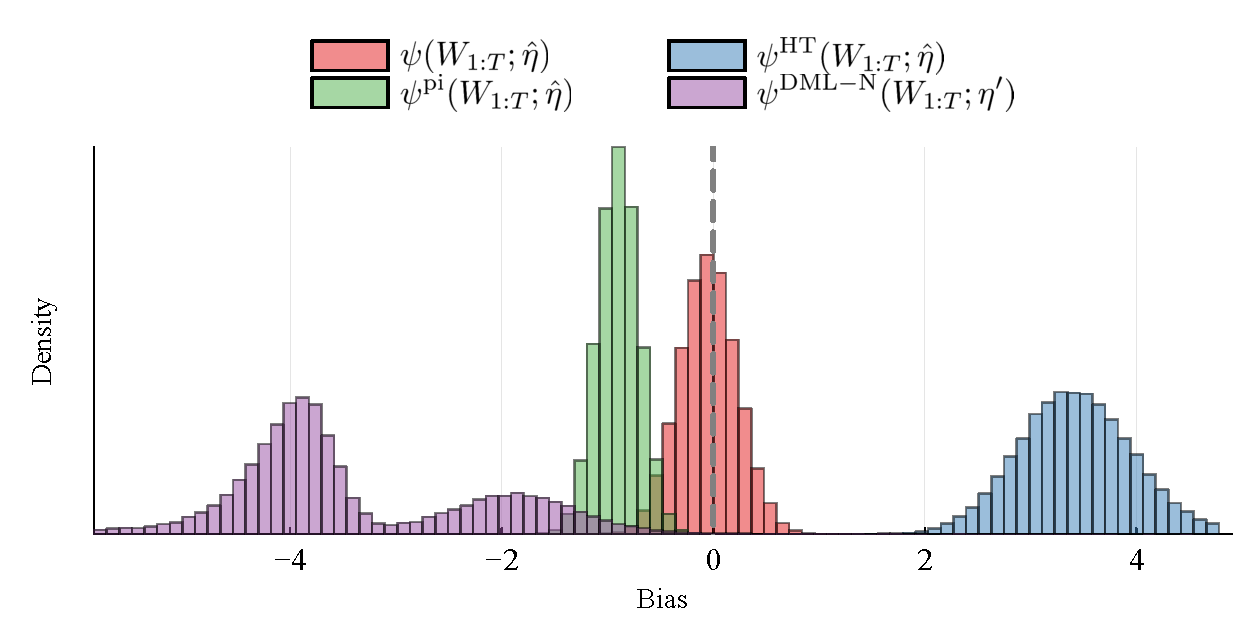
\includegraphics[width=0.65\textwidth]{image/direct_effect.pdf}
    \caption{Hình 2 --- Phân phối ước lượng điểm của ADE. Các phương pháp bỏ qua \(H_t\) (HT, Plug-in, Naive DML) bị chệch nặng; chỉ DML4SSI và SSAC tập trung quanh vạch 0 (giá trị thực).}
    \label{fig:ade_bias}
\end{figure}

\begin{figure}[H]
    \centering
    \begin{minipage}[t]{0.48\textwidth}
        \centering
        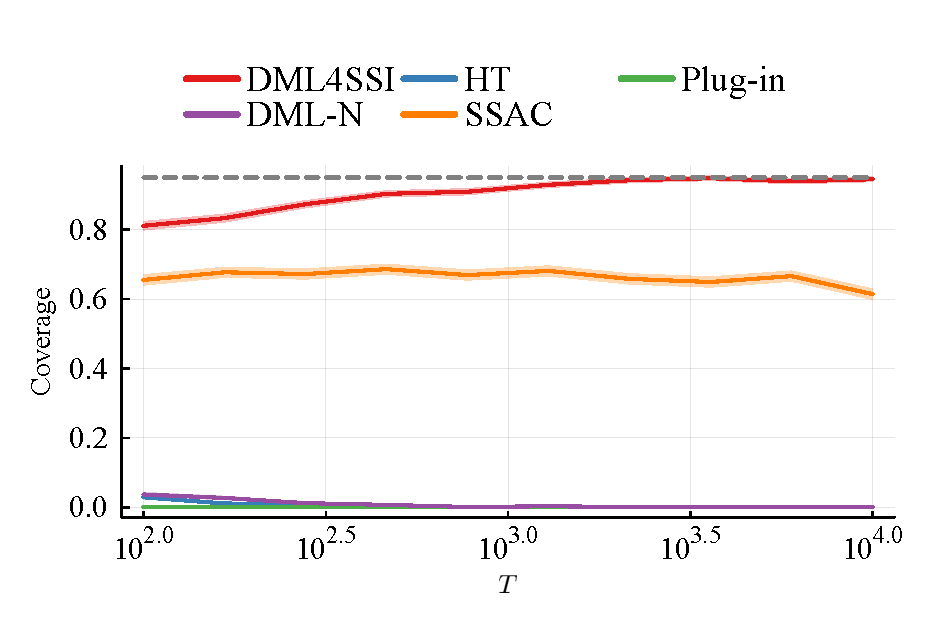
\includegraphics[width=\textwidth]{image/coverage_vs_sample_size.pdf}
    \end{minipage}
    \hfill
    \begin{minipage}[t]{0.48\textwidth}
        \centering
        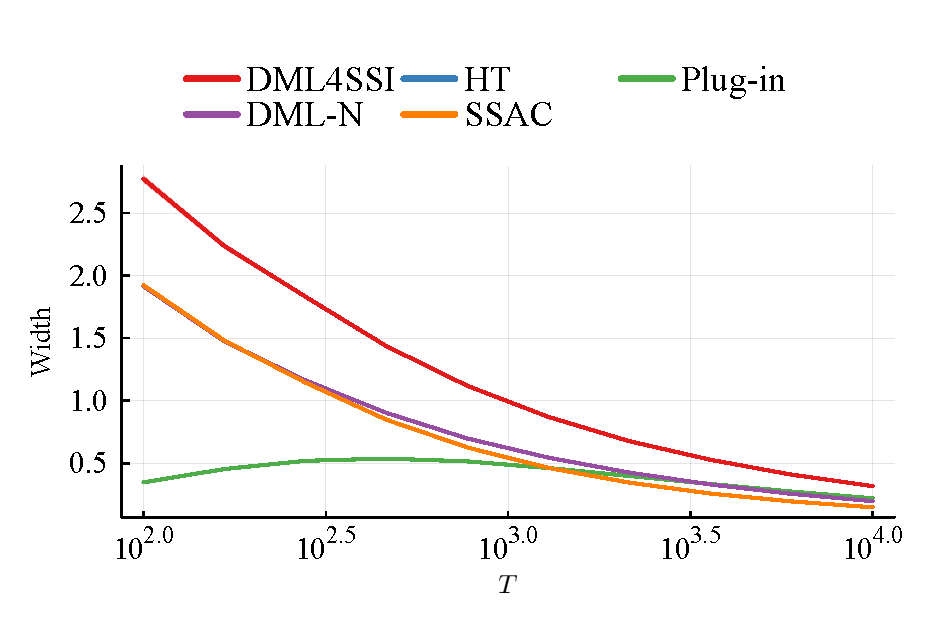
\includegraphics[width=\textwidth]{image/width_vs_sample_size.pdf}
    \end{minipage}
    \caption{Hình 3 --- Độ phủ (trái) và Độ rộng (phải) của khoảng tin cậy 95\% cho ADE theo cỡ mẫu \(T\). Chỉ DML4SSI hội tụ đến mức phủ chuẩn 95\%; SSAC bị kẹt ở 60--70\% do đánh giá thấp phương sai.}
    \label{fig:ade_ci}
\end{figure}

\begin{itemize}
    \item \textbf{DML4SSI:} Độ phủ nhanh chóng hội tụ về mức chuẩn \textbf{95\%} khi \(T\) tăng.
    \item \textbf{SSAC:} Tuy không chệch về điểm ước lượng nhưng \textbf{đánh giá thấp phương sai} do bỏ qua hiệp phương sai chuỗi thời gian --- khoảng tin cậy quá hẹp, độ phủ thực tế chỉ đạt 60--70\% và \textit{không bao giờ} hội tụ về 95\% dù tăng \(T\).
    \item Các phương pháp naive (HT, Plug-in, Naive DML): độ phủ xấp xỉ 0.
\end{itemize}

\textbf{Kết luận:} Chỉ \textbf{DML4SSI} đồng thời đảm bảo ước lượng điểm không chệch \textit{và} khoảng tin cậy đạt mức phủ chuẩn 95\%.

\subsection{Thực nghiệm cho GATE trong Switchback (Hình 4, 5 \& 6)}

\subsubsection{Thiết lập mô phỏng}

Tương tự phần ADE, với \(f^*\) là hàm phi tuyến của \(D_t, X_t, H_t\) và độ dài switchback \(\ell = 2m\). Bộ ước lượng đề xuất được so sánh với:

\begin{itemize}
    \item Các phương pháp naive (HT, Plug-in, Naive DML) --- như trong bài toán ADE.
    \item \textbf{Switchback HT (SB)} (Bojinov et al., 2022): bộ ước lượng không chệch được thiết kế đặc biệt cho thử nghiệm switchback.
\end{itemize}

\subsubsection{Kết quả}

\begin{figure}[H]
    \centering
    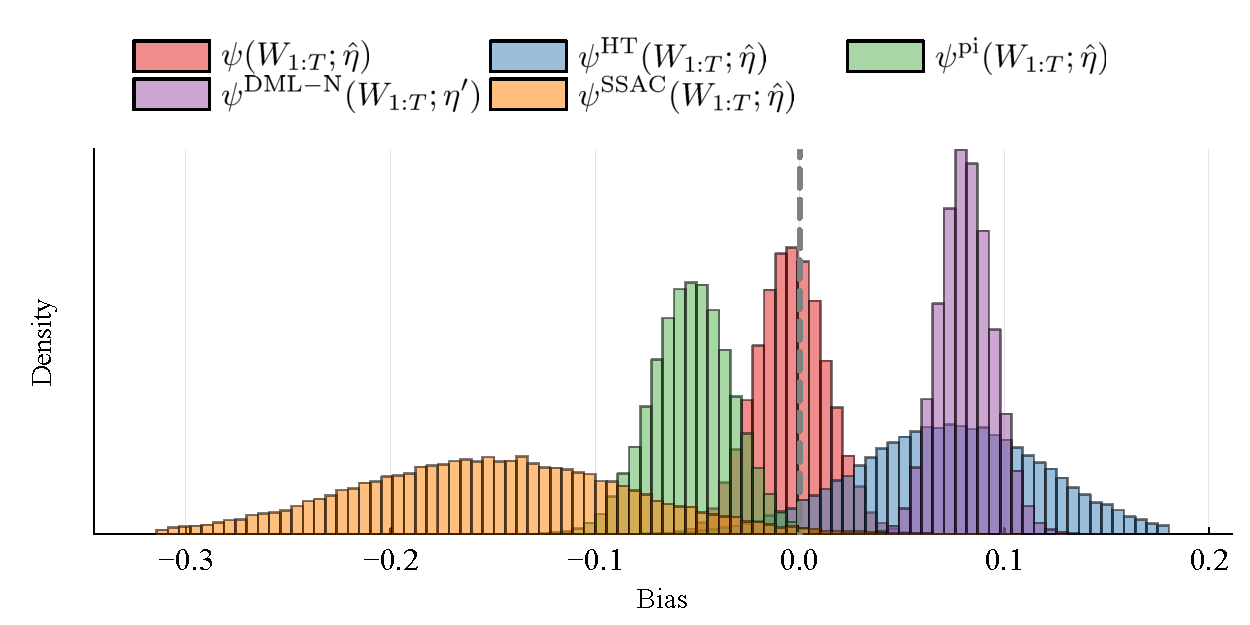
\includegraphics[width=0.65\textwidth]{image/switchback_vs_naive.pdf}
    \caption{Hình 4 --- Phân phối ước lượng điểm của GATE trong Switchback: DML4SSI so với các phương pháp naive. Các phương pháp naive bị chệch nặng; DML4SSI tập trung xung quanh giá trị thực.}
    \label{fig:gate_bias}
\end{figure}

\begin{figure}[H]
    \centering
    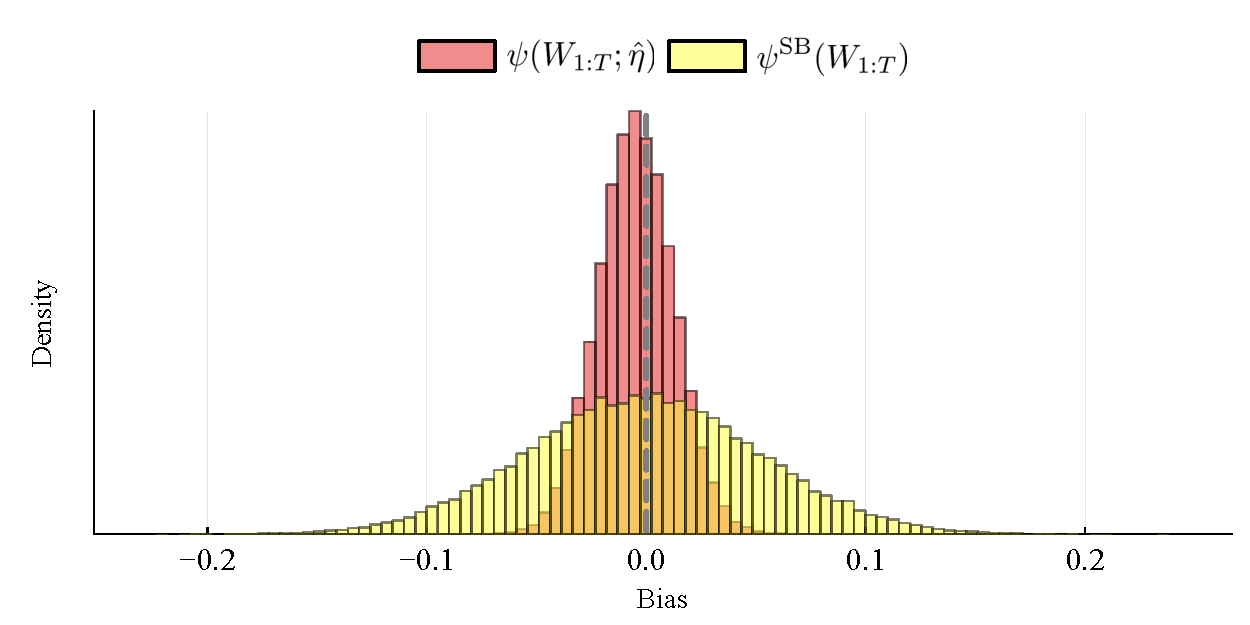
\includegraphics[width=0.65\textwidth]{image/switchback.pdf}
    \caption{Hình 5 --- So sánh DML4SSI với Switchback Horvitz-Thompson (SB). Cả hai đều không chệch nhưng DML4SSI có phương sai thấp hơn đáng kể (phân phối nhọn hơn).}
    \label{fig:gate_vs_sb}
\end{figure}

Cả hai phương pháp đều \textit{không chệch} (phân phối cân tâm tại giá trị thực), nhưng \textbf{DML4SSI có phương sai thấp hơn đáng kể}. Hai lý do chính:
\begin{enumerate}
    \item Học máy giải thích biến động qua covariate và trạng thái chung, loại bỏ nhiễu không cần thiết.
    \item Phương pháp SB bắt buộc phải bỏ đi \(m\) bước đầu mỗi khối chuyển giao, trong khi DML4SSI tận dụng toàn bộ dữ liệu thông qua thành phần Regression Adjustment.
\end{enumerate}

\begin{figure}[H]
    \centering
    
\includegraphics[width=0.75\textwidth]{image/gate_coverage_width.png}
    \caption{Hình 6 --- Độ phủ (trái) và Độ rộng (phải) của khoảng tin cậy 95\% cho GATE theo cỡ mẫu \(T\). DML4SSI hội tụ về 95\%; SB đạt 100\% do phương sai ước lượng quá bảo thủ, dẫn đến khoảng tin cậy rộng hơn DML4SSI từ 3 đến 7,5 lần.}
    \label{fig:gate_ci}
\end{figure}

\begin{itemize}
    \item \textbf{Độ phủ (Coverage):} DML4SSI nhanh chóng hội tụ về mức chuẩn 95\%. SB luôn đạt 100\% do ước lượng phương sai quá bảo thủ.
    \item \textbf{Độ rộng (Width):} Khoảng tin cậy của SB \textbf{rộng gấp 3 đến 7,5 lần} so với DML4SSI.
\end{itemize}

\textbf{Ý nghĩa kinh tế:} Khả năng thu hẹp khoảng tin cậy của DML4SSI cho phép doanh nghiệp \textbf{tiết kiệm 3--7,5 lần cỡ mẫu hoặc thời gian chạy A/B test} để đưa ra quyết định với cùng mức độ tin cậy.

\section{Kết luận và Thảo luận}

\subsection{Tổng kết đóng góp}

Bài báo ``Double Machine Learning for Causal Inference under Shared-State Interference'' của Hays và Raghavan (MIT, 2025) đề xuất một khung lý thuyết và thực hành mới để suy luận nhân quả trong các hệ thống có nhiễu loạn trạng thái chung (SSI). Ba đóng góp chính gồm:

\begin{enumerate}
    \item \textbf{Mô hình hóa SSI tổng quát:} Định nghĩa chính thức khái niệm shared-state interference thông qua chuỗi Markov với trạng thái chung \(H_t\), bao phủ nhiều ứng dụng thực tế (thị trường, hệ thống gợi ý, gọi xe công nghệ).

    \item \textbf{Mở rộng định lý DML:} Chứng minh định lý suy luận tiệm cận hợp lệ cho dữ liệu phụ thuộc theo chuỗi thời gian. Thay thế cross-fitting K-fold bằng auxiliary data (dưới geometric ergodicity) hoặc block cross-fitting với khoảng đệm (dưới \(m\)-dependence).

    \item \textbf{Ứng dụng thực tiễn:} Cung cấp hai bộ ước lượng cụ thể (ADE và GATE), được kiểm chứng qua mô phỏng cho thấy DML4SSI vừa không chệch vừa đạt độ phủ khoảng tin cậy chuẩn 95\%, trong khi tất cả các phương pháp thay thế đều thất bại ít nhất một tiêu chí.
\end{enumerate}

\subsection{Hạn chế}

\begin{itemize}
    \item \textbf{Yêu cầu dữ liệu phụ trợ:} Giải pháp auxiliary data đòi hỏi có sẵn tập dữ liệu \(W_{\text{aux}}\) độc lập với tập suy luận --- điều này có thể không khả thi trong mọi bối cảnh.
    \item \textbf{Cần biết \(m\):} Trong trường hợp \(m\)-dependence (switchback), cần biết hoặc ước lượng được khoảng thời gian \(m\) để \(H_t\) phai nhạt hoàn toàn.
    \item \textbf{Chỉ xét đối xử nhị phân và kết quả thực:} Bài báo hiện giới hạn ở \(D_t \in \{0, 1\}\) và \(Y_t \in \mathbb{R}\).
\end{itemize}

\subsection{Hướng mở rộng}

Các hướng nghiên cứu tiếp theo có thể gồm:
\begin{itemize}
    \item Mở rộng sang đối xử liên tục (continuous treatment).
    \item Xét trường hợp trạng thái chung không quan sát được (latent shared state).
    \item Phát triển phương pháp ước lượng \(m\) từ dữ liệu (đã được đề cập trong bài báo switchback).
    \item Ứng dụng trong các thí nghiệm A/B test trực tuyến với dữ liệu lớn thực tế.
\end{itemize}

\input{ref/references.tex}

\end{document}
